\documentclass[11pt]{article}
  \renewcommand{\baselinestretch}{1.05}
  \usepackage{amsmath,amsthm,verbatim,amssymb,amsfonts,amscd,graphicx}
  \usepackage{graphics}
  \usepackage{url}
  \usepackage[utf8]{inputenc}
  \graphicspath{{images/}}
  \topmargin0.0cm
  \headheight0.0cm
  \headsep0.0cm
  \oddsidemargin0.0cm
  \textheight23.0cm
  \textwidth16.5cm
  \footskip1.0cm
  \theoremstyle{plain}
  \newtheorem{theorem}{Theorem}
  \newtheorem{corollary}{Corollary}
  \newtheorem{lemma}{Lemma}
  \newtheorem{proposition}{Proposition}
  \newtheorem*{surfacecor}{Corollary 1}
  \newtheorem{conjecture}{Conjecture}
  \newtheorem{question}{Question}
  \theoremstyle{definition}
  \newtheorem{definition}{Definition}


   \begin{document}

  \title{Kuvien tunnistus neuroverkoilla}
  \author{Teemu Sarapisto}
  \maketitle

  \section{Alkuhommat}


  Neuroverkot yleistyneet viimeaikoina koska GPU:t. Neuroverkkojen lisäkerroksien hyöty löydetty (deep learning). Perustuvat osittain biologisten neuroverkkojen toimintaperiaatteisiin. Konvoluutioneuroverkot erittäin hyviä klassifioimaan kuvia. \cite{Goodfellow-et-al-2016}


  \section{Neuroverkkojen rakenne}
  \subsection{Yksi neuroni / perseptroni}
   %kappaleessa 3 rojanista hyvää juttua \cite{Rojas96}

   %http://neuralnetworksanddeeplearning.com/chap1.html keksi parempi lähde
   % oliko varmasti 50-luvulla?
   Keinotekoiset neuroverkot koostuvat useista keinotekoisista neuroneista. Neuroneista yksinkertaisimpia ovat 50-luvulla kehitetyt "perseptronit". Perseptronit ottavat vastaan binäärisiä (syötteen arvo voi olla joko 0 tai 1) syötteitä $x_1$, $x_2$, ..., ja kunkin syötteen vaikutusta ulostuloarvoon (output?) säädetään siihen liittyvällä painolla $w_i$. Perseptronilla on yksi ulostuloarvo, 0 tai 1 joka riippuu siitä, onko summa $\Sigma x_i * w_i$ yli, vai alle jonkin valitun kynnysarvon. Muut keinotekoiset neuronit ovat paljolti perseptroneja vastaavia, esimerkiksi hyvin yleisesti käytetyssä sigmoidisessa neuronissa syöte- ja ulostuloarvoina käyvät mitkä tahansa reaaliluvut välillä 0-1, ja ulostulon määrää aktivaatiofunktioksi kutsuttu kaava (TODO: bias arvon "b" selitys kaavasta) $\sigma(w_i*x_i + b)$, jossa $\sigma(z) = 1/(1-e^{-z}))$\cite{Nielsen-neural}

   \subsection{Verkko neuroneja}

   TODO: piirrä oma kuva / keksi jostain royalty free, tää on täältä http://neuralnetworksanddeeplearning.com/images/tikz11.png
   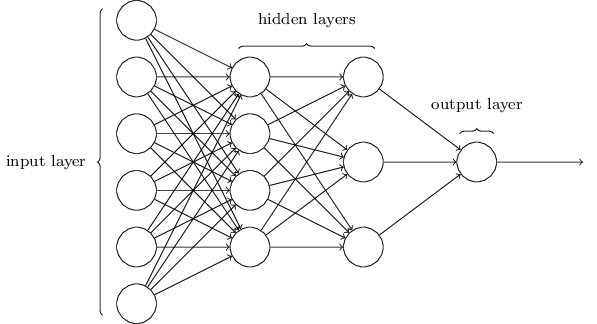
\includegraphics[scale=0.5]{basic-neuralnet}

   [under-construction.gif]

   Yksinkertaisimmassa neuroverkkorakenteen omaavat feedforward (suomennos?) neuroverkot muodostetaan tasoittain, jossa jokaisen neuroverkon tason neuronit saavat syötteenään niitä edeltävien tasojen neuroneiden ulostuloarvot. Poikkeuksena ensimmäinen taso (kuvassa vasemmanpuoleisimpana), joihin verkon alkuperäinen syöte koodataan jollakin halutulla tavalla. Esimerkiksi haluttaessa syöttää 64x64 kuva neuroverkolle, voidaan syötekerroksena käyttää 64x64 neuronin kerrosta, johon kuvan pikselien väriarvot koodataan.

   (For example, the convolutional networks used for object recognition from photos are a specialized kind of feedforward network)
   
   \section{Neuroverkkojen oppiminen / opettaminen}
   - backpropagation, gradient descent, cost function

   - overfitting

   - (regularization, dropout)

   - weight initialization

   \section{Erilaiset neuroverkot}
   - Olemassa esim RNN, CNN

   - CNN toimii hyvin kuvien tunnistamiseen. Millaisia CNN:t ovat tarkemmin
   \section{Kuvien tunnistus (konvoluutioneuroverkoilla)}
   - local receptive fields, shared weights/biases, pooling

   \renewcommand{\refname}{Lähteet}
   \bibliographystyle{ieeetr}
   \bibliography{test}

  \end{document}